\documentclass[a4paper,12pt]{article}
\addtolength{\oddsidemargin}{-1.cm}
\addtolength{\textwidth}{2cm}
\addtolength{\topmargin}{-2cm}
\addtolength{\textheight}{3.5cm}
\newcommand{\HRule}{\rule{\linewidth}{0.5mm}}
\makeindex

\usepackage{longtable}
\usepackage[pdftex]{graphicx}
\usepackage{makeidx}
\usepackage{hyperref}
\usepackage{verbatim}
\hypersetup{
    colorlinks=true,
    linkcolor=blue,
    filecolor=magenta,      
    urlcolor=cyan,
}


% define the title
\author{IMAPKD}
\title{ Testing}
\begin{document}
\setlength{\parskip}{6pt}

% generates the title
\begin{titlepage}

\begin{center}
% Upper part of the page       

\includegraphics[width=1\textwidth]{./University_of_Pretoria_Logo.PNG}\\[0.4cm]  
\textsc{\LARGE COS 301}\\[0.9cm]
\textsc{\LARGE Department Of Computer Science}\\[0.3cm]

%Title

\HRule \\[0.4cm]
{ \huge \bfseries Testing Document}\\[0.1cm]
\HRule \\[0.4cm]  

% Group Members 

\begin{minipage}{0.4\textwidth}
\begin{flushleft} \large

\emph{\Large Group Members:}\\[0.4cm]    
\emph{}\\
{\Large Diana {Obo}} \\
\emph{}\\
\emph{}\\
{\Large Priscilla {Madigoe}}\\
\emph{}\\
\emph{}\\
{\Large Kudzai {Muranga}} \\
\emph{}\\
\emph{}\\
{\Large Sandile {Khumalo}}\\
\emph{}\\
\emph{}\\

\end{flushleft}
\end{minipage}
\begin{minipage}{0.4\textwidth}
\begin{flushright} \large

\emph{ \Large Student numbers:} \\[0.4cm]  
\emph{}\\
{\Large u13134885}\\
\emph{}\\
\emph{}\\
{\Large u13049128}\\
\emph{}\\
\emph{}\\
{\Large u13278012}\\
\emph{}\\
\emph{}\\
{\Large u12031748}\\
\emph{}\\
\emph{}\\

\end{flushright}
\end{minipage}

% bottom section of title page

{\large \today}
\end{center}
\end{titlepage}
\renewcommand{\thesection}{\arabic{section}}

\newpage
\begin{center}
\textsc{\Large IMPAKD link}\\[0.5cm]
For further references see \href{https://github.com/u13278012/IMPAKD/}{gitHub}.
\today
\end{center}
\newpage
\tableofcontents{}

\newpage
\section{addPropertyTest.js file}
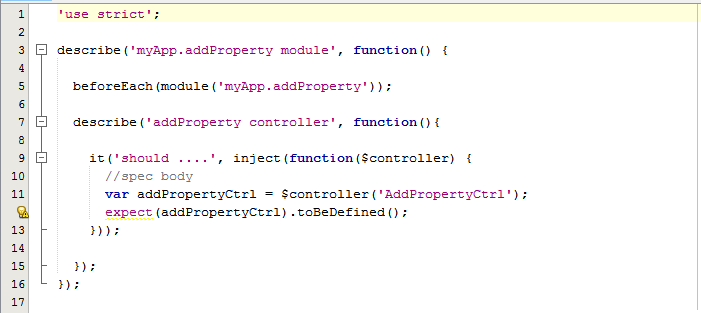
\includegraphics[width=1\textwidth]{./addProperty_test.PNG}\\[0.4cm] 

\section{homeTest.js file}
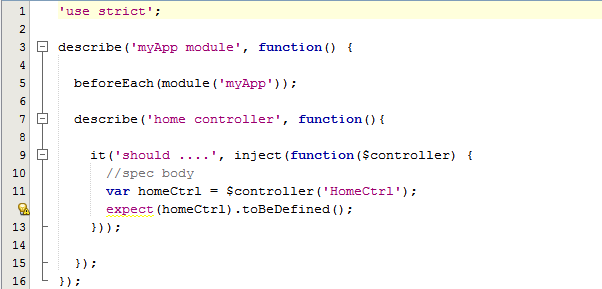
\includegraphics[width=1\textwidth]{./home_test.PNG}\\[0.4cm]

\section{propertyDetailsTest file}
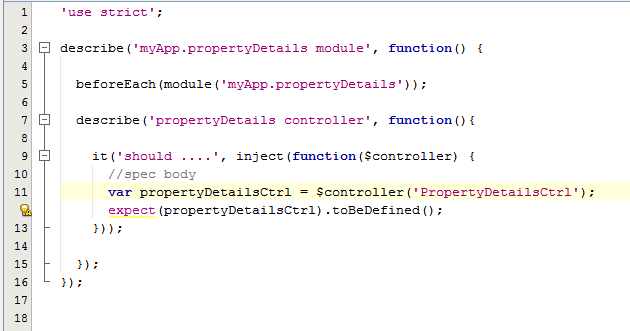
\includegraphics[width=1\textwidth]{./propertyDetails_test.PNG}\\[0.4cm]

\section{Terminal to run test}
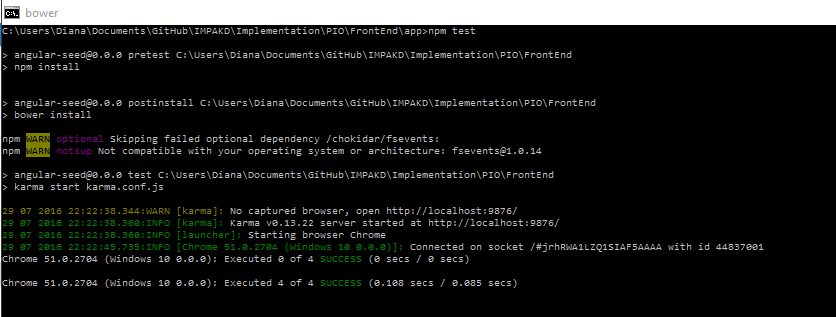
\includegraphics[width=1\textwidth]{./karma.PNG}\\[0.4cm]
\end{document}

